\documentclass{standalone}

\usepackage{graphics}
\usepackage[dvipsnames,svgnames]{xcolor}

\usepackage{tikz,pgf,pgfplots,circuitikz}
\pgfplotsset{compat=1.15}
\usetikzlibrary{shapes.symbols,intersections,arrows.meta,angles,calc,3d,decorations.pathmorphing}
\usepackage[compat=1.1.0]{tikz-feynhand}

\usepackage{amssymb,amsfonts,amsthm,mathtools}
\usepackage{physics,braket,bm}

\begin{document}

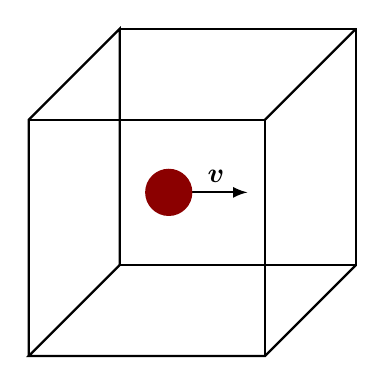
\begin{tikzpicture}
  % Draw the cube
  \draw[thick] (0,0,0) -- (3,0,0) -- (3,3,0) -- (0,3,0) -- cycle; % Front face
  \draw[thick] (0,0,0) -- (0,0,3) -- (3,0,3) -- (3,0,0); % Bottom face
  \draw[thick] (0,0,0) -- (0,3,0) -- (0,3,3) -- (0,0,3); % Left face
  \draw[thick] (0,3,3) -- (3,3,3) -- (3,0,3); % Back face
  \draw[thick] (3,3,0) -- (3,3,3); % Top right edge
  \draw[thick] (0,3,3) -- (3,3,3); % Top back edge
  \draw[thick] (3,0,3) -- (3,3,3); % Right back edge

  % Draw the arrows inside the cube
  \draw[thick, -latex] (1.2, 1.5, 1.5) -- (2.2, 1.5, 1.5); % Horizontal arrow
  
  % Draw the circle inside the cube
  \fill[thick, DarkRed] (1.2, 1.5, 1.5) circle (0.3);

  % Label the rotation
  \node at (1.8, 1.7, 1.5) {$\bm{v}$};
\end{tikzpicture}

\end{document}


